

\newcommand{\ysc}[0]{1}
\newcommand{\xsc}[0]{1}




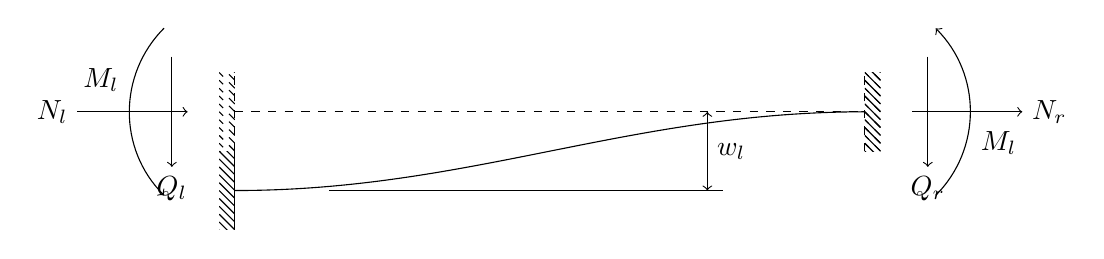
\begin{tikzpicture}[yscale =\ysc, xscale=\xsc, radius=1.5cm]

\draw[dashed](0,0) -- (8,0);
\draw[dashed](0, -0.5) -- (0, 0.5);
\draw[dashed](8, -0.5) -- (8, 0.5);

\begin{scope}
\clip (-0.2,-0.5) rectangle (0,0.5);
\draw[dashed](0, -0.7) -- (-0.2, -0.5);
\draw[dashed](0, -0.6) -- (-0.2, -0.4);
\draw[dashed](0, -0.5) -- (-0.2, -0.3);
\draw[dashed](0, -0.4) -- (-0.2, -0.2);
\draw[dashed](0, -0.3) -- (-0.2, -0.1);
\draw[dashed](0, -0.2) -- (-0.2, -0.0);
\draw[dashed](0, -0.1) -- (-0.2,  0.1);
\draw[dashed](0,  0.0) -- (-0.2,  0.2);
\draw[dashed](0,  0.1) -- (-0.2,  0.3);
\draw[dashed](0,  0.2) -- (-0.2,  0.4);
\draw[dashed](0,  0.3) -- (-0.2,  0.5);
\draw[dashed](0,  0.4) -- (-0.2,  0.6);
\draw[dashed](0,  0.5) -- (-0.2,  0.7);
\end{scope}

\begin{scope}[xshift=8.2cm, yshift=-0.2cm]
\clip (-0.2,-0.3) rectangle (0,0.7);
\draw[dashed](0, -0.7) -- (-0.2, -0.5);
\draw[dashed](0, -0.6) -- (-0.2, -0.4);
\draw[dashed](0, -0.5) -- (-0.2, -0.3);
\draw[dashed](0, -0.4) -- (-0.2, -0.2);
\draw[dashed](0, -0.3) -- (-0.2, -0.1);
\draw[dashed](0, -0.2) -- (-0.2, -0.0);
\draw[dashed](0, -0.1) -- (-0.2,  0.1);
\draw[dashed](0,  0.0) -- (-0.2,  0.2);
\draw[dashed](0,  0.1) -- (-0.2,  0.3);
\draw[dashed](0,  0.2) -- (-0.2,  0.4);
\draw[dashed](0,  0.3) -- (-0.2,  0.5);
\draw[dashed](0,  0.4) -- (-0.2,  0.6);
\draw[dashed](0,  0.5) -- (-0.2,  0.7);
\draw[dashed](0,  0.6) -- (-0.2,  0.8);
\draw[dashed](0,  0.7) -- (-0.2,  0.9);
\end{scope}


\draw(0,-0.5) -- (0,-1.5);
\draw(0, -1) .. controls (3, -1) and (5, 0) .. (8, 0);


\begin{scope}[yshift=-1cm]
\clip (-0.2,-0.5) rectangle (0,0.5);
\draw(0, -0.7) -- (-0.2, -0.5);
\draw(0, -0.6) -- (-0.2, -0.4);
\draw(0, -0.5) -- (-0.2, -0.3);
\draw(0, -0.4) -- (-0.2, -0.2);
\draw(0, -0.3) -- (-0.2, -0.1);
\draw(0, -0.2) -- (-0.2, -0.0);
\draw(0, -0.1) -- (-0.2,  0.1);
\draw(0,  0.0) -- (-0.2,  0.2);
\draw(0,  0.1) -- (-0.2,  0.3);
\draw(0,  0.2) -- (-0.2,  0.4);
\draw(0,  0.3) -- (-0.2,  0.5);
\draw(0,  0.4) -- (-0.2,  0.6);
\draw(0,  0.5) -- (-0.2,  0.7);
\end{scope}

\begin{scope}[xshift=8.2cm, yshift=-0.2cm]
\clip (-0.2,-0.3) rectangle (0,0.7);
\draw(0, -0.7) -- (-0.2, -0.5);
\draw(0, -0.6) -- (-0.2, -0.4);
\draw(0, -0.5) -- (-0.2, -0.3);
\draw(0, -0.4) -- (-0.2, -0.2);
\draw(0, -0.3) -- (-0.2, -0.1);
\draw(0, -0.2) -- (-0.2, -0.0);
\draw(0, -0.1) -- (-0.2,  0.1);
\draw(0,  0.0) -- (-0.2,  0.2);
\draw(0,  0.1) -- (-0.2,  0.3);
\draw(0,  0.2) -- (-0.2,  0.4);
\draw(0,  0.3) -- (-0.2,  0.5);
\draw(0,  0.4) -- (-0.2,  0.6);
\draw(0,  0.5) -- (-0.2,  0.7);
\draw(0,  0.6) -- (-0.2,  0.8);
\draw(0,  0.7) -- (-0.2,  0.9);
\end{scope}

\draw[<-, color=black](-0.6, 0) -- (-2,0)node[left]{$N_l$};
\draw[->, color=black](-0.8, 0.7) -- (-0.8, -0.7)node[below]{$Q_l$};
\draw[<-, color=black](-0.9,-1.06) arc[start angle=225, end angle=135];
\node at (-1.7, 0.4){$M_l$};

\draw[->, color=black](8.6, 0) -- (10,0)node[right]{$N_r$};
\draw[->, color=black](8.8, 0.7) -- (8.8, -0.7)node[below]{$Q_r$};
\draw[<-, color=black](8.9,1.06) arc[start angle=45, end angle=-45];
\node at (9.7, -0.4){$M_l$};


\draw[<->](6, 0) -- (6, -1);
\draw[color=black](1.2,-1) -- (6.2, -1);
\node at (6, -0.5)[right]{$w_l$};

\end{tikzpicture}
